\subsection{Субъектно-ориентированная модель рекомендательной
системы}
Одой из первых РС, в которой была применена
СОМ для решения задач, --- это РС, разработанная компанией
GroupLens \cite{grouplens}.

СОМ проводят анализ предпочтений
пользователей. Отфильтровываются те пользователи, чьи предпочтения не близки.
Если пользователи близки
по предпочтениям, то между ними выполняется отношение близости, и тогда
информация о таких пользователях используется для решения задачи. В
исследованиях, посвященных СОМ, такие пользователи называются
соседями \cite{neighbor-cf}.
Для РС интернет-магазина близость по предпочтениям может
выражаться, к примеру, тем, что пользователи приобретают одни и те
же товары (то есть объекты) \cite{e-commerce}.

В СОМ характеристиками пользователей являются объекты,
значениями характеристик --- значения $\rho(u, i)$, которые определяют
предпочтения пользователей.
В общем случае соседями считаются те пользователи,
кто одинаково оценивает одни и те же объекты, что во введенной
терминологии запишется в следующем виде:
\begin{equation}
	\label{user-sim1}
	u \ru v \Leftrightarrow \forall i: \exists \rho(u,i) \wedge
	\exists \rho(v,i) \text{ верно, что } |\rho(u,i) -
	\rho(v,i)| \le \varepsilon_p,
\end{equation}
где $\varepsilon_p$ --- некоторая малая фиксированная величина.

Определим отношение близости на основании меры близости
$\du: U \times U \rightarrow [0,1]$. Считается,
что если мера близости между пользователями больше некоторого порогового
значения, то пользователи являются соседями  \cite{threshold1, threshold2,
threshold3,threshold4,threshold5}:
\begin{equation}
	\label{user-sim2}
	u \ru v \Leftrightarrow \du(u,v) \ge \Delta_u, \Delta_u \in
	[0,1]
\end{equation}
Стоит отметить, что при разработке СОМ необходимо подбирать
параметры $\du$ и $\Delta_u$ так, чтобы близкие пользователи по определению
\ref{user-sim1}, были близки по определению \ref{user-sim2}:
важность подбора таким образом параметров будет описана в главах, посвященных
анализу коллаборативной фильтрации и последующих после текущей главы.

Правило вывода $\Pi_C$ в СОМ основано на утверждении, которое
гласит, что если в прошлом пользователи были близки по вкусам,
то и в будущем они будут близки по вкусам \cite{ub-assumption}.
Во введенной
терминологии данное утверждение примет следующий вид:
\begin{equation}
\label{srs-assert}
u_a \ru u \text{ выполняется на } P_0 \Rightarrow u_a
\ru u \text{ выполняется на } P_{\bot}
\end{equation}
Во время проведения тестов множеством будущего выступает тестовое множество,
множеством настоящего --- обучающее.

Правило вывода СОМ основывается
на эвристическом утверждении \cite{cfrs}, которое гласит :
\begin{assert}\label{assertSRS1}
пользователи, схожие по предпочтениям в прошлом, будут схожи и в будущем.
\end{assert}
Поэтому утверждение
во введенной терминологии запишется следующим образом:
\begin{equation*}
	\forall i_0:
	|\rho(u,i_0) - \rho(v,i_0)| \le \varepsilon_p
	\Rightarrow \forall i_{\bot} |\rho(u,i_{\bot}) - \rho(v,i_{\bot})|
	\le \varepsilon_p,
\end{equation*}

Правило вывода $\Pi_C$ в СОМ задается следующей формулой:
\begin{equation}
	\label{srs-pi}
	u \in U, (u_a \ru u) \Rightarrow |\rh(u_a, i_{\bot}) - \rho(u_a, i_{\bot})|
	\le \varepsilon_p, \rh(u_a, i_{\bot}) = f_p(\{\rho(u, i_{\bot})\}).
\end{equation}
Правило вывода СОМ говорит о том, что если пользователи $u$ являются
соседями для пользователя $u_a$, то оценки близости $\rho(u_a, i_{\bot}), \rho(u, i_{\bot})$
коррелируют, поэтому
неизвестное значение $\rho(u_a, i_{\bot})$ можно функционально определить по
значениям $\{\rho(u, i_{\bot})\}$, то есть прогнозная функция является функцией от
значений оценок близости соседей.

Данная модель используется, в основном, для решения задачи $pred$.
%Рассмотрим, как правило вывода применяется для решения задач.
%%%%%%%%%%%%%%%%%%%%%%%%%%% TOPN %%%%%%%%%%%%%%%%%%%%%%%%%%%%%%%%%%%%%%%%%%

\subsubsection{Задача $topN$}
Схема решения задачи $topN$ заключается в построении кластера соседей
$\nut = \{u: u_a \ru u\}$ активного пользователя $u_a$, который выступает в
роли центра кластера. После того, как кластер был
построен, выбирается $N$ объектов, которые близки для большинства
пользователей.

Это решение основано на правиле вывода $\Pi_C$ --- пусть объект $i$ близок
для большинства пользователей кластера $\nut$: $(\frac{1}{|\nut|} \sum \limits_{u \in
\nut} \rho(u,i)) \ge \Delta_{\R}$, а функциональная зависимость $f_p$
прогнозной функции $\rh$ определяется средним значением оценок близостей
соседей $\rho(u,i)$. Тогда $\rh(u_a, i) = f_p(\{\rho(u, i)\})
> \Delta_{\R}$, и тогда можно утверждать, что $u_a \R i$. $N$ таких объектов
составляет решение задачи $topN$.

Опишем возможную\footnote{Модели могут отличаться такими параметрами, как,
например, функция $\du$, поэтому нижеописанная модель является одной из
возможных}
модель CОМ
\footnote{
	На данном этапе без оценки качества $\mathcal{E}_{topN}$
	}
 и на ее примере решим
задачу $topN$  \cite{amazon-linden}.%TODO: set cite

\begin{itemize}
	\item $c_X(u_a) = (x_1, x_2, ..., x_n)$
\begin{equation*}
  x_i =
  \begin{cases}
	1, &\text{если $u_a \R i$}\\
	  0, &\text{иначе}
  \end{cases}
\end{equation*}
	Это распространенный способ представления контента,
	где координаты соответствуют объектам
		 \cite{topn1}.
	Данный способ представления
	информации о пользователях заимствован из информационного поиска
	 \cite{e-commerce,empirical-cf,ir4};
	\item $c_Y$ не определяется, так как с объектами в СОМ работа не проводится;
	\item $\di(u_a,u) =\cos(\angle(c_X(u_a),c_X(u)))$.
\end{itemize}

Чтобы сформировать кластер соседей, производится линейный поиск соседей
на множестве пользователей \cite{amazon-item2item}. Для построения результирующего
множества просуммируем контенты (данная операция
допустима, так как контент представляет из себя вектор) соседей,
и выберем те координаты $i$, которые обладают наибольшими значениями
и $(i, \rho(u_a,i)) \not \in P_0$.


На рисунке (\ref{dia:nut}) изображена блок-схема алгоритма
построения кластера соседей $\nut$, которой соответствует псевдокод
, представленный на изображении <<Построение множества соседей для активного
		пользователя $u_a$ при решении задачи $topN$>>
(\ref{alg:nut}).
\begin{figure}[htb]
	\caption{Блок-схема алгоритма построения кластера $\nut$}
\begin{center}
	\label{dia:nut}
 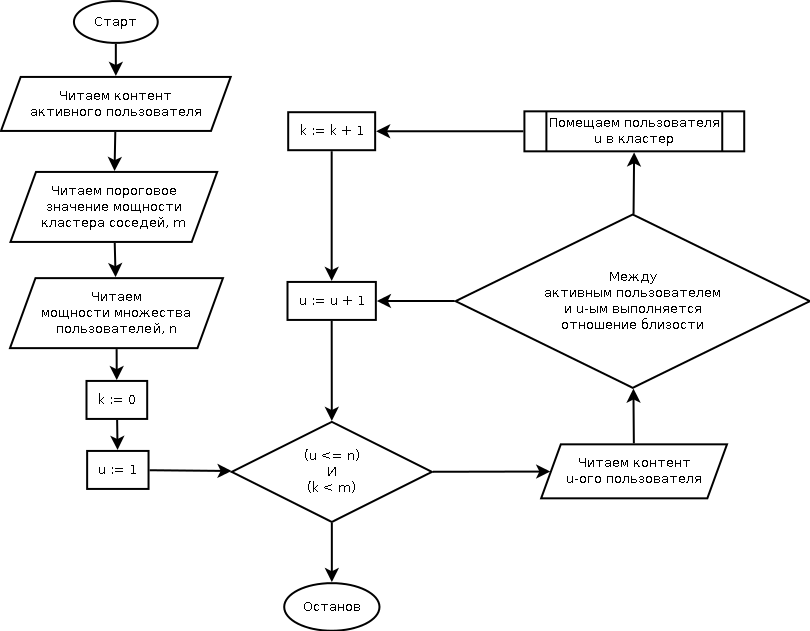
\includegraphics[width=7in,height=8in]{pics/algs/nut.png}
\end{center}
\end{figure}

\begin{figure}[htbp]
	%\begin{algorithm}
		\caption{Построение множества соседей для активного
		пользователя $u_a$ при решении задачи $topN$}
		\label{alg:nut}
		\begin{algorithmic}[1]
			\State $\nut \gets \varnothing$
			\State $k \gets 0$
			\For {$u \gets 1 \to |U|$}
			\If{$u_a \ru u$}
			\State $\nut \gets \nut \bigcup \{ u \}$
			\State $k \gets k + 1$
			\EndIf
			\If{$k > M$}\Comment{Ограничение на размер множества соседей}
			\State Стоп
			\EndIf
			\EndFor
		\end{algorithmic}
	%\end{algorithm}
\end{figure}


На рисунке (\ref{dia:topn-srs}) изображена блок-схема решения задачи $topN$ в
$COM$, которой соответствует псевдокод, представленный на изображении <<Стандартный алгоритм решения задачи $topN$>>  (\ref{alg:topn-srs}).
\begin{figure}[htb]
	\caption{Решение задачи $topN$ в $COM$}
	\begin{center}
		\label{dia:topn-srs}
		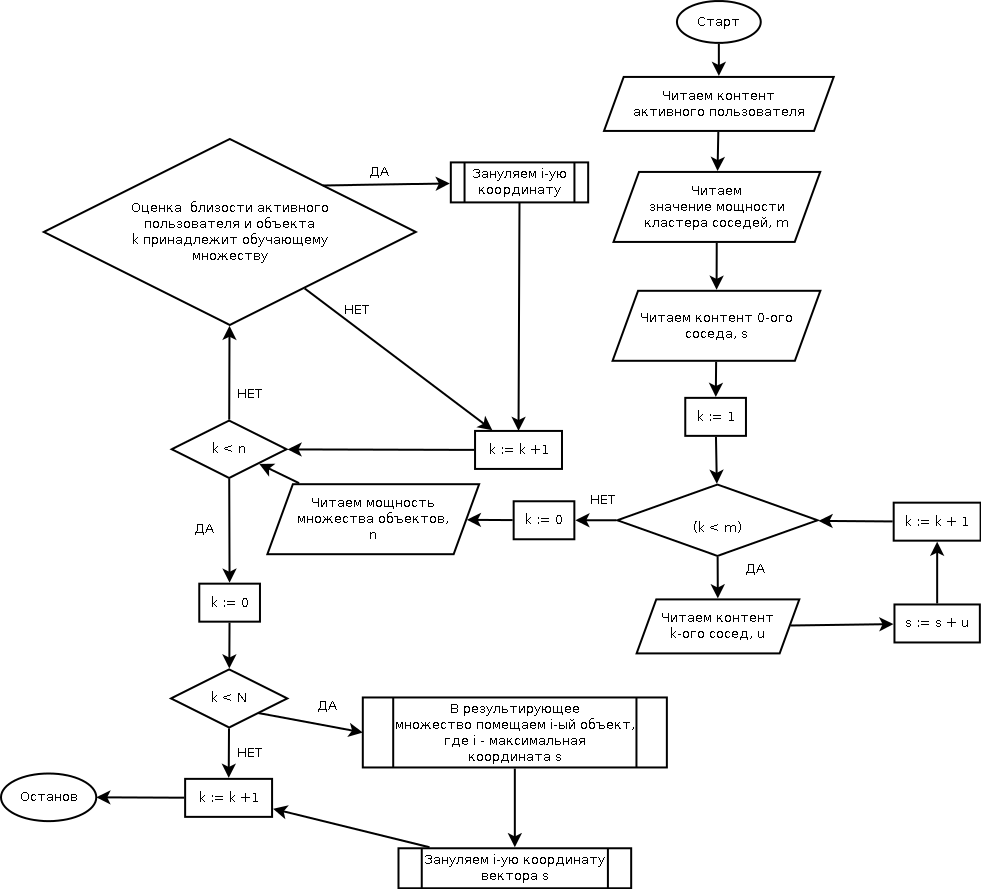
\includegraphics[width=7in,height=8in]{pics/algs/topn-srs.png}
	\end{center}
\end{figure}

\begin{figure}[htbp]
	%\begin{algorithm}
		\caption{Стандартный алгоритм решения задачи $topN$}
		\label{alg:topn-srs}
		\begin{algorithmic}[1]
			\State $s \gets \sum \limits_{u \in \nut} u$ \Comment{Вектор-сумма}
			\For {$i \gets 1, i \le |I|$}
			\If {$\exists \rho(u_a,i)$} \Comment{Если активный пользователь уже оценил
			объект, то он должен отсутствовать в результирующем множестве}
			\State $s_i \gets 0$ \Comment{Зануляем $i$-ую координату}
			\EndIf
			\EndFor
			\State $\overline{P}^a_{\bot} \gets \varnothing$
			\State $I_{topN} \gets \varnothing$
			\For {$k \gets 1, k \le N$}
			\State $i \gets \underset{i} {\mathrm{\max}}$ $s$
			\State $I_{topN} \gets I_{topN} \bigcup \{i\}$
			\State $\overline{P}^a_{\bot} \gets \overline{P}^a_{\bot} \bigcup
			\{ 0 \}$ \Comment{Для решения задачи нужно составить множество объектов, а не
			определить близость, поэтому $\rho(a,i)=0$, так как тогда $\forall
			\epsilon_0:$ $u_a \R i$}
			\State $s_i \gets 0$
			\State $k \gets k + 1$
			\EndFor
		\end{algorithmic}
	%\end{algorithm}
\end{figure}


\subsubsection{Задача прогнозирования}
Подобно задаче $topN$, для решения задачи $pred$ \cite{cfrs, cf-expert,
rs-handbook, toward,coscial-rec-survey, user-item-cf,rs-cf}
строится кластер соседей, центром которого является активный пользователь
$u_a$, однако в кластер входят не только те пользователи, между которыми
и активным выполняется отношение близости, но и такие, которые оценили
прогнозируемый объект $i_{\bot}$:
$\nup = \{u: u_a \ru u \wedge \rho(u,i_{\bot}) \in P_0\}$. Такое дополнительное
условие накладывается для того, чтобы по известным $\rho(u, i_{\bot}), u \in \nup$
определить неизвестную $\rho(u,i_{\bot})$.
Следуя утверждению СОМ (\ref{assertSRS1}), $\forall$ $u \in \nup$ выполняется $|\rho(u_a,i_{\bot}) -
\rho(u,i_{\bot})| \le
\varepsilon_p$.
Для того, чтобы рассчитать прогнозную оценку,
вычисляется значение некоторой прогнозной функции $f_p$
от оценок, поставленных прогнозируемому объекту соседями:
\begin{equation}
	\rh(u_a,i_{\bot}) = f_p(\{ \rho(u,i_{\bot}): u \in \nup \})
\end{equation}

На рисунке (\ref{dia:nup}) изображена блок-схема алгоритма
построения кластера соседей $\nup$, которой соответствует псевдокод
(\ref{alg:nup}).
\begin{figure}[htb]
	\caption{Блок-схема алгоритма построения кластера $\nup$}
\begin{center}
	\label{dia:nup}
 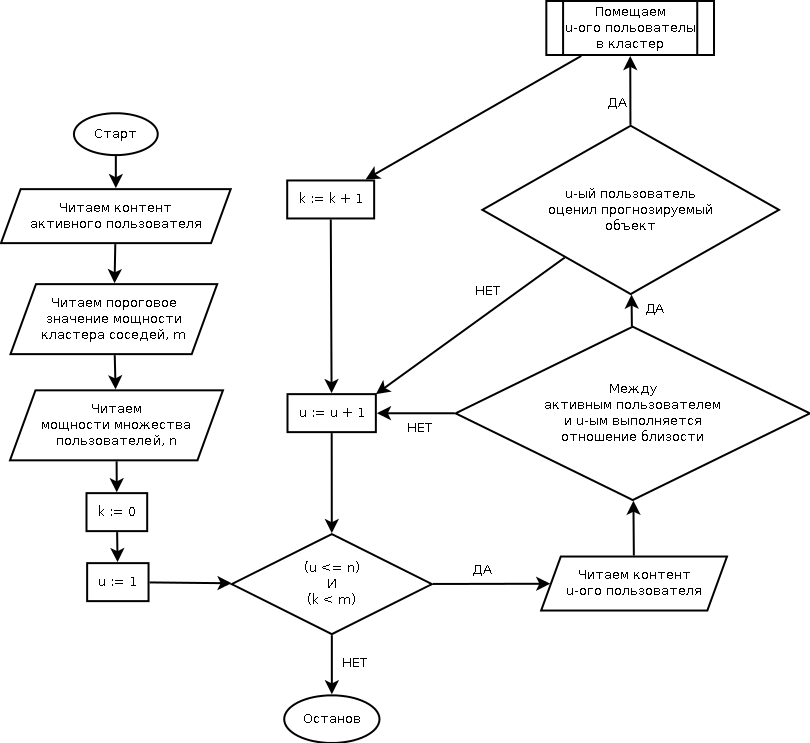
\includegraphics[width=7in,height=8in]{pics/algs/nup.png}
\end{center}
\end{figure}

\begin{figure}[htb]
	%\begin{algorithm}
		\caption{Построение множества соседей для активного
		пользователя при решении задачи прогнозирования в СОМ}
		\label{alg:nup}
		\begin{algorithmic}[1]
			\State $\nup \gets \varnothing$
			\State $k \gets 0$
			\For {$u \gets 1 \to |U|$}
			\If{($u_a \ru u$) $\wedge$ $(\exists$ $\rho(u, i_{\bot}))$}
			\State $\nup \gets \nup \bigcup \{ u \}$
			\State $k \gets k + 1$
			\EndIf
			\If{$k > M$}\Comment{Ограничение на размер множества соседей}
			\State Стоп
			\EndIf
			\EndFor
		\end{algorithmic}
	%\end{algorithm}
\end{figure}

Стандартный алгоритм решения задачи $pred$ в СОМ производится
в две итерации, которым соответствует псевдокод, представленный на изображении <<Стандартный алгоритм решения задачи прогнозирования в СОМ>>
 (\ref{alg:p-srs}):
\begin{enumerate}
	\item формирование кластера соседей $\nup$ (\ref{alg:nup});
	\item вычисление прогнозной функции по множеству оценок $\{\rho(u, i_{\bot}): u
		\in \nup\}$.
\end{enumerate}

\begin{figure}[htb]
	\caption{Стандартный алгоритм решения задачи прогнозирования в СОМ}
	\label{alg:p-srs}
		\begin{algorithmic}[1]
			\State $\nup$ \Comment{Формируем кластер соседей}
			\State $\rh(u_a, i_{\bot}) \gets f(\{\rho(u, i_{\bot}): u
			\in \nup\})$ \Comment{Вычисляем прогнозную функцию}
		\end{algorithmic}
\end{figure}


\subsubsection{Функции вычисления прогнозной оценки}
Приведем примеры распространенных функций $f_p$, которые используются для
вычисления значения прогнозной функции по значениям $\rho(u, i), u \in \nup$.
\begin{itemize}
  \item Среднее  \cite{surveyCf}:
  \begin{equation}
	\label{middle-pred}
    \frac{1}{|\nup|} \cdot \sum \limits_{u \in \nup} \rho(u,i_{\bot}).
  \end{equation}
  \item Среднее взвешенное \cite{surveyCf}:
  \begin{equation}
	  \label{weighted-pred}
    \overline{\rho^a} +
    \frac{ \sum \limits_{u \in \nup} \du(u_a,u) \cdot (\rho(u,i_{\bot}) -
	  \overline{\rho^u}) }
{ \sum \limits_{u \in \nup} | \du(u_a,u) | }
  \end{equation}
  $\overline{\rho^a}$ --- среднее значение близости активного пользователя,
		$\overline{\rho^u}$ --- среднее значение близости пользователя $u$.
Вычитание средней оценки близости призвано устранить эффект,
который накладывается от характера пользователя:
		лояльные пользователи ставят оценки близости не ниже определенной,
строгие пользователи --- наоборот \cite{norm, rs-handbook}.

Приведенные способы вычисления прогнозной оценки являются распространенными, но не единственными.
К примеру, компания Ringo \cite{ringo} не использовала в своей системе веса,
а среднее значение меры сходства соседей. Однако
метод среднего взвешенного является не только простым и распространенным,
но и согласуется с
теорией общественного выбора, ее обоснованиями человеческого поведения, ---
первичными принципами коллаборативной фильтрации  \cite{cfrs,bellcore}.
\end{itemize}

%%%%%%%%%%%%%%%%%%%%%%%%%%%%%%%%%%%%%%%%%%%%%%%%%%%%%%%%%
\subsubsection{Меры сходства}
Приведем примеры распространенных функций, которые используются в качестве меры
сходства.
\begin{itemize}
\item Коэффициент корреляции Пирсона\label{pearson}:
\begin{equation}
	\du(u,v)\frac{\sum \limits_{i \in I_{\bigcap}}(\rho(u,i) - \overline{\rho}^u) \cdot
	(\rho(v,i) - \overline{\rho}^v)}
                {\sqrt{\sum \limits_{i \in I^u}(\rho(u,i) - \overline{\rho})^u \cdot
                    \sum \limits_{i \in I^v}(\rho(v,i) - \overline{\rho}^v)^2}}
\end{equation}
\begin{equation*}
	I^a = \{i: (i, \rho(a,i)) \in P^a_0\}, a \in \{u,v\},P^a_0 = \{\rho(a, i_0)\}
\end{equation*}
\begin{equation*}
	I_{\bigcap} = I^u \bigcap I^v
\end{equation*}
\item Косинус угла между контентами.
	Для применения этой меры сходства необходимо представлять
контенты как элементы векторного пространства, в котором координата
		соответствует объекту и равна нулю, если пользователь не оценивал
		данный объект.
\begin{equation}
cos(\angle(u,v) = \frac{\sum \limits_{ i \in I_{\bigcap} } \rho(u,i) \cdot \rho(v,i)}{
\sqrt{ \sum \limits_{i \in  I^u } (\rho(u,i))^2 } \cdot \sqrt{ \sum \limits_{ i \in I^v} (\rho(u,i))^2 }},
\end{equation}
\end{itemize}


\subsubsection{Примеры решения задач}
Рассмотрим примеры решения задач в СОМ.
\paragraph{Данные}
\begin{itemize}
\item $N=2$ --- для задачи $topN$ требуется определить 2 топовых объекта;
\item $i_{\bot} = 7$ --- для задачи прогнозирования необходимо спрогнозировать оценку на объект 7;
\item $\mathcal{S} = \{0,1;0,2;0,3;0,4;0,5\}$ --- оценки принадлежат относительной шкале от 1 до 5. Если оценка равна 0; то пользователь не
ставил оценку на данный объект.
\item $|I| = 10$
\item Контенты пользователей --- вектор оценок, где $i-ая$ координата соответствует $i$-ому объекту.
  \begin{itemize}
    \item $a =   (0,5; 0,2; 0,4; 0,3; 0,5; 0,0; 0,0; 0,0; 0,0; 0,0)$
    \item $u_1 = (0,5; 0,2; 0,5; 0,0; 0,4; 0,2; 0,5; 0,0; 0,0; 0,0)$
    \item $u_2 = (0,4; 0,3; 0,5; 0,0; 0,4; 0,0; 0,0; 0,4; 0,5; 0,2)$
    \item $u_3 = (0,2; 0,5; 0,2; 0,4; 0,3; 0,0; 0,0; 0,5; 0,4; 0,0)$
    \item $u_4 = (0,0; 0,0; 0,0; 0,0; 0,0; 0,2; 0,0; 0,3; 0,5; 0,5)$
    \item $u_5 = (0,4; 0,2; 0,0; 0,0; 0,4; 0,2; 0,5; 0,5; 0,0; 0,0)$
  \end{itemize}
\item $\Delta_{\R} = 0,49$
\item В качестве меры сходства будем использовать коэффициент корреляции
	Пирсона (\ref{pearson}).
\item
  \begin{equation}
    \du(u_1,u_2) > 0.8 \Rightarrow u_1 \ru u_2
  \end{equation}
\end{itemize}
\paragraph{Задача $topN$}
\begin{enumerate}
\item Составим множество соседей мощности 2. Для этого рассчитаем меру сходства между активным пользователем и другими:
  \begin{itemize}
  \item $\du(u_a,u_1) = 0,94 \Rightarrow u_1 \in \nut$
  \item $\du(u_a,u_2) = 0,57$
  \item $\du(u_a,u_3) = -0,85$
  \item $\du(u_a,u_4) = \varnothing$
  \item $\du(u_a,u_5) = 0,81 \Rightarrow u_5 \in \nut$
  \end{itemize}
\item $s = \sum \limits_{u \in \nut} u = (0,9; 0,4; 0,5; 0,0; 0,8; 0,4; 1,0; 0,5; 0,0; 0,0)$
\item Зануляем значения координат, для которых $\rho(u_a, i) \in P_0: s =
	(0,0; 0,0; 0,0; 0,0; 0,0;0,4; 1,0; 0,5; 0,0; 0,0)$
\item $I_{topN} = \{ 7, 8 \}$
\end{enumerate}
\paragraph{Задача прогнозирования}
При решении предыдущей задачи было составлено множество соседей.
Определим прогноз по оценкам этих соседей:
\begin{equation}
f_p(u_a,7) =  0,38 + \frac{ 0,94 \cdot (0,5 - 0,38) + 0,81 \cdot (0,5 - 0,36)}{
	0,94 + 0,81 } = 0,55
\end{equation}

%%%%%%%%%%%%%%%%%%%%%%%%%%% PREDICT %%%%%%%%%%%%%%%%%%%%%%%%%%%%%%%%%%%%%%%%%%
%%%%%%%%%%%%%%%%%%%%%%%%%%% PREDICT FUNCTIONS %%%%%%%%%%%%%%%%%%%%%%%%%%%%%%%%%%%%%%%%%%
